\documentclass[11pt, a4paper, titlepage]{article}
\usepackage[onehalfspacing]{setspace} 
\usepackage{fullpage}
\usepackage{helvet}
\renewcommand{\familydefault}{\sfdefault}
\usepackage{graphicx}
\graphicspath{./images/}
\usepackage{float} % needed for [H]
\usepackage{titlesec}
\usepackage{lineno}
\usepackage[round]{natbib}
\usepackage[margin=2cm]{geometry}
\usepackage{hyperref}
\hypersetup{
	colorlinks,
	linkcolor={red!50!black},
	citecolor={blue!50!black},
	urlcolor={blue!80!black}
}
\linenumbers
\onehalfspacing
\usepackage{pgfgantt}


\begin{document}
    \begin{titlepage}
    \begin{center}
            {\large IMPERIAL COLLEGE LONDON}
    \end{center}
    
    \vspace*{\fill}
    
    \begin{center}
        {\Huge 
    	 Geographical variations in the sensitivity of terrestrial biodiversity to anthropogenic pressures}
        \\[2in]
        Author: Kayleigh Greenwood, MSc CMEE (kg21@ic.ac.uk)
        \bigskip
        \newline
       Internal Supervisor: Dr James Rosindell, Imperial College London (j.rosindell@imperial.ac.uk)
       \bigskip
       \newline
        External Supervisor: Dr Joss Wright, University of Oxford (joss.wright@oii.ox.ac.uk)
        \bigskip
        \newline

        25/08/2022
        \\[2in]
        
        {\bfseries A thesis submitted in partial fulfilment of the requirements for the degree of Master of Science at Imperial College London \newline \newline Submitted for the MSc in Computational Methods in Ecology and Evolution }

        

    
	\end{center}
    \vspace{\fill}
    
    \end{titlepage}
	\section*{Declaration}
	\begin{center}
	Data was obtained from existing online databases, and therefore I was not responsible for data processing or cleaning. \newline
	Were any mathematical models developed by you or by your supervisor? \newline
	What role, if any, did your supervisor play in developing the analyses presented?
	\end{center}
	\newpage
	
	\section*{Abstract}
	 To our knowledge, very little prior research has studied geographic differences in sensitivity to biodiversity pressures. Hence, studying geographical variation in  sensitivity would be useful in comparing the impact of pressures on global biodiversity.
	
	\newpage
	\tableofcontents
	
	\newpage
	
    \section*{Introduction}
    \addcontentsline{toc}{section}{Introduction}
    	
    \subsection*{Overview}
    \addcontentsline{toc}{subsection}{Overview}
    %Para 1: biodiversity is important. pressures act on biodiversity
   	 Ecosystems with intact biodiversity provide services such as clean air and pollination, which makes the earth habitable for humans \citep{leemans2003millennium}. Loss of such biodiversity leads to unstable environments which are less resistant to change. Biodiversity loss diminishes ecosystem productivity \citep{duffy2017biodiversity} and threatens all life on earth, including human well-being \citep{diaz2006biodiversity}. Biodiversity is impacted by both natural and anthropogenic pressures \citep{nobel2020anthropogenic}, however any mention of 'biodiversity pressures' in this study refers only to the latter. Understanding the impacts of anthropogenic pressures on biodiversity is important for creating accurate environmental policies and conservation strategies, and therefore more effective ones. \newline
   	 
   	%Para: Sustainable business and investments
   	 Aside from traditional efforts for protecting biodiversity, another response to the biodiversity crisis \citep{ogar2020science} is the beginning of a global movement towards sustainable business and biodiversity-conscious investment \citep{pri2020}\citep{worldeconomicforum2020}\citep{wwf2020}. Creating a tool which assesses the overall biodiversity impact of a company can help guide investors. This is something that various parties are currently developing \citep{worldbenchmarkingalliance_2022}\citep{iccs_2020}. The World Benchmarking Alliance is using an approach centred around researching published materials from top companies. Dissimilarly, 'Benchmark for Nature' is a project which is using open-source data from news articles that have been web-scraped, in an effort to gain the maximum amount of data possible about the links that companies/sectors have with each biodiversity pressure. Benchmark for Nature aims to use data science to develop a framework for assessing investment impacts on biodiversity \citep{iccs_2020}, similar to the ESG framework currently in place. The ESG information currently available only assesses an investments' impact on the environment, but not on living nature and biodiversity. The purpose of the project is to better inform investors so that more biodiversity-conscious decisions can be made, in an effort to aid the biodiversity loss crisis \citep{gasu2021review}, and also indirectly, the climate \citep{shin2022actions}.   \newline
   	 
   	%Para :  Geographical variations in both biodiversity and its' pressures
   	 Assessing the impact that investments/companies have on biodiversity involves calculating their contributions towards the main pressures (e.g. deforestation, pollution etc.). It is also useful to know where in the world these effects are taking place, so that we know how much biodiversity is at risk. The worlds' biodiversity is not equally distributed, it varies geographically \citep{gaston2000global} \citep{ricklefs2004comprehensive} \citep{mcrae2017diversity}. Various direct and indirect pressures correlate with this variation in biodiversity \citep{sunday2015species}, \citep{ament2019compatibility} \citep{Velde2022}. The magnitude of pressures acting on biodiversity also varies across regions/biomes \citep{millennium2005ecosystems} \citep{sala2000global}, and as do their spatial couplings \citep{bowler2020mapping} meaning the pressures on biodiversity are not equally distributed geographically. An assumption in some literature and models of biodiversity response is that whilst magnitude of pressures varies, sensitivity to these pressures is constant geographically \citep{sala2000global}, however there is no research to support this assumption. Despite any patterns observed in magnitude of pressures, there will always be variation in biodiversity response to such pressures due to species' varying sensitivities \citep{bowler2020mapping}. In the context of Benchmark for Nature's tool, web articles are unlikely to mention the exact species that a company is having an impact on, and is more likely to mention the general region the impact is taking place, meaning regional insights into sensitivity would be useful. For this reason, the question that has been raised is whether sensitivity to biodiversity pressures differs geographically. Insights about geographical variations in biodiversity sensitivity at regional levels (e.g. country, continent) would be the most useful for tools like Benchmark for Nature, but have not been adequately studied. A possible explanation for the inadequate research in this area is that the rise in global biodiversity impact tools (like benchmark for nature) have created a demand for higher level (e.g. country, continent) data that previously had no use because species-level data was sufficient. Having regional information on biodiversity sensitivity will allow the impact of pressures on biodiversity to be better estimated in situations where it is not clear which species are being impacted, and only the area of impact is known. Rather than just including how biodiversity in general is likely to respond, it would be more useful to know how local biodiversity in that specific region is likely to respond.  \newline
   	 
   	 \subsection*{Interspecific and intertaxon sensitivity}
   	 \addcontentsline{toc}{subsection}{Interspecific and intertaxon sensitivity}
   	%Para: Introducing species varying sensitivities and why they aren't enough
   	 Although there is no available database about how biodiversity sensitivity differs geographically, it is well known that interspecies responses to biodiversity pressures vary \citep{foden2013identifying}. Given also that each region of the world comprises different combinations of species groups \citep{goethem2021biodiversity}, there is reason to believe that sensitivity to biodiversity pressure could vary depending on location. One of the papers which studied interspecific sensitivity to environmental pressures \citep{louette2010bioscore}, developed a set of sensitivity scores for European species, determining which species will benefit from, be indifferent to, or be negatively affected by environmental change. This 'Bioscore' study used such sensitivity scores to create a tool for predicting the effect of a policy change on Europe's biodiversity. The proportion of affected species in each region was used to map the effects of a change in each biodiversity pressure. The sensitivity scores for each species were obtained from published literature about individual species' responses to change in different environmental variables. The BioScore tool suggests that even if the magnitude of a biodiversity pressure is constant across Europe, biodiversity's response can still vary according to country, due to varying sensitivity of the species within such country. This study is a predictive tool based on published studies about individual species, and a wider-breadth study is necessary to observe worldwide variances in countries sensitivities to biodiversity pressures. The BioScore tool's predictions support the concept that country-wide differences in sensitivity could exist. \newline
   	 
   	 % Para: Between taxa variation and intra specific variation
   	 Sensitivity to environmental change also varies between taxa and should not be assumed to be constant \citep{sunday2015species}. This between-taxa variation further supports the concept that sensitivity to biodiversity pressures could vary on larger scales. Given that there have been differences in sensitivity to pressures found at both the species, and taxa level, then grouping species into even broader categories (such as country) could continue to show such differences. This supports the idea that researching differences between regional sensitivity, could contribute to more accurate predictions of how biodiversity pressures impact biodiversity. Another reason that studying sensitivity at a broader scale than species is useful, links to intra-specific variation. It is common practice among both meta-analyses and projects, such as the IUCN redlist ,to extrapolate findings about a population's sensitivity to the species on the whole \citep{iucn2001iucn} \citep{buckley2012functional}. High intraspecific variation exists in response to biodiversity pressures like climate change \citep{mclean2018high} \citep{both2004large} \citep{mayor2016assessing}. This could mean that extrapolating findings about one population of a species to the species on the whole could be problematic. \newline
   	 
   	 
   	 \subsection*{Geographical differences in sensitivity}
   	 \addcontentsline{toc}{subsection}{Geographical differences in sensitivity}
   	 %Para: studies that support the hypothesis of geographic differences in sensitivity
   	 An understanding of the sensitivity of biodiversity of an entire region could be a more accurate metric for studies of a global scale. Sensitivity to habitat loss can vary according to location (study site) \citep{mayor2016assessing}, further supporting the concept that sensitivity could differ geographically. \newline
   	 
   	 %para: biome sensitivities
   	 Biodiversity sensitivity differs between biomes for the following biodiversity pressures; pollution (nitrogen exceedance) \citep{alkemade2009globio3}, land use change and climate change \citep{newbold2020tropical}. The most sensitive biomes were tropical biomes \citep{barlow2016anthropogenic} with the least sensitive being temperate and boreal biomes \citep{newbold2020tropical} \citep{cazalis2021mismatch} \citep{barlow2016anthropogenic}. Despite geographical variations in sensitivity existing between biomes, little is known about continental differences. Biomes are unequally distributed between the continents, with South America having a higher percentage cover of tropical forest than any other continent, and Europe having the lowest closely followed by North America \citep{wade2003distribution}.  Because of the aforementioned sensitivity differences between biomes, it could be that Europe and North America will have lower sensitivity to biodiversity pressures than other continents, with South America being the most sensitive. However, of the minimal research that has studied continental differences, findings contradict this hypothesis as they showed tropical forest biodiversity sensitivity to be higher in Asia than in other regions (Americas and Africa). \citep{gibson2011primary}. 
   	
   	\subsection*{Research aims}
   	\addcontentsline{toc}{subsection}{Research aims}
   	
   	%Para 9: Conclusion
   	 Given that anthropogenic impact on the environment is worldwide \citep{plumptre2021might}, the question should be raised of whether the geographic location of biodiversity pressures affects their impact on global biodiversity. The understanding of variations in biodiversity sensitivity, along with many other aspects of biodiversity, has knowledge gaps which desperately need filling \citep{pereira2012global}. If such geographic differences exist, they should be taken into account when attributing biodiversity-related merit to investments. To widen the scope of impact outside of the Benchmark for Nature project, taking into account geographic variations in sensitivity to biodiversity pressures could make estimates about biodiversity impact more accurate. Better understanding of biodiversity pressures will aid a better understanding of the implications of investments (and other policies) on natural ecosystems.  This research aims to investigate whether the location of a pressure affects its' level of impact on biodiversity which is important more so now than ever \citep{ceballos2015accelerated}. Add to this paragraph a brief description of how I will conduct my study. State hypotheses. \newline

	%include section about why i'm looking at whether COUNTRIES WITHIN A CONTINENT are significantly different to COUNTRIES IN ANOTHER CONTINENT
	In order to find out which level of sensitivity insight would be useful (e.g. country, continent), I will assess the articles already collected by the Benchmark project to determine the most commonly mentioned (and therefore most useful) location terminology.
	
	
   	\newpage

    \section*{Methods}
	\addcontentsline{toc}{section}{Methods}
	 % very very very important that if i'm using BII, i talk about measuring biodiversity INTACTNESS instead of measuring biodiversity.
	\subsection*{Overview}
	\addcontentsline{toc}{subsection}{Overview}

	The focus of this study is on anthropogenic biodiversity pressures only. Anthropogenic pressures on biodiversity are typically grouped, in the current literature, into 5 main pressures; climate change, land use change, pollution, invasive species and overexploitation. In order to assess whether sensitivity to each pressure varies by country, data was needed in the form of time series (how each of these pressures had been changing in each country over time, as well as how each country's biodiversity had been changing over time). The time series of biodiversity in a country was compared to the time series of a pressure on biodiversity in that country, in order to extract a 'sensitivity score' for each country to assess any effect of geography. \newline
	
	First, each pressure's geographic relationship with biodiversity was assessed in isolation. It is important to look at individual biodiversity pressures, as opposed to an aggregated pressure on biodiversity, because the pressures have spatial differences \citep{steffen2015planetary}, meaning the geographical magnitude of each pressure varies. Therefore in order to understand how countrys differ in their responses to biodiversity pressures, it must be taken into account the magnitude of each pressure that each country experiences. \newline
	\subsection*{Data}
	\addcontentsline{toc}{subsection}{Data}
	
	BD data = 18 years, 240 countries
	The variable chosen to represent biodiversity was biodiversity intactness. The National History Museum's (NHM) Biodiversity Intactness Index (BII)\citep{phillips2021} was chosen as it presents biodiversity in the context of how many original species remain (relative to reference populations). The NHM's Index is the best for this project as the database used is that of the PREDICTS project, which more geographically representative than other datasets \citep{purvis2018modelling}. This allows for direct comparison of these changes, with the changes in anthropogenic pressures. Historical BII data spanned 1970 - 2014. \newline
	
	Climate data = 120 years, 230 countries
	Time series data for climate change was obtained in the form of annual average temperature for each country. The temperature dataset chosen was from the World Bank's Climate Change Knowledge Portal. This dataset was chosen because it contains comprehensive historical data, providing an annual average temperature for every year from 1900 until 2020. \newline
	
	Built Land data = 4 years, 249 countries (years is big problem!)
	To represent land use change, the dataset used was The Global Human Settlement Layer data package \citep{JRC117104}. The data contains information on built-up area change over time, which is the variable chosen to represent land use change. Collective land use change is difficult to quantify from land use statistics. Although satellite data is available to categorise land cover type over time, calculating annual land use change from the proportion of each land cover type is not necessarily accurate, as land use change can be multi-directional. Current studies assessing the impact of land use change on biodiversity are often meta-analyses or use a natural regional situation as the reference land type \citep{de2013land} as opposed to observing direct impacts of land use change. Statistics \newline
	
	GHG data = 31 years, 63 countries (countries is problem!)
	With the focus being on terrestrial biodiversity, greenhouse gases (GHG) were used as the representative variable for 'pollution' as a biodiversity pressure. The dataset used to access GHG emissions for each country over time was the 'National Inventory Submissions' section of the United Nations - Climate Change website \citep{united nations}. GHG emissions are presented both including and excluding 'Land Use, Land-Use Change and Forestry (LULUCF)' related emissions data. When assessing pollution and biodiversity links in isolation, LULUCF was included. However, when modelling all biodiversity pressures together, LULUCF was tested for collinearity with the land use change variable, and consequently included/excluded. \newline
	
	The OECD.stat website was used to download the land use change and pollution data. \newline
	
	Overexploitation was excluded for multiple reasons. Firstly, overexploitation is the vaguest of the main pressures, and is usually used in the context of fishing (marine biodiversity being beyond the scope of this project). One of the most relevant aspects of overexploitation to is deforestation, which is (maybe remove this part depending on methods) already represented in the variable used for land use change. Though there are other aspects of overexploitation that would be relevant (e.g. illegal wildlife trading), there are no databases/studies available representing overexploitation by country.

	\subsection*{Method 1: model for each country}
	\addcontentsline{toc}{subsection}{Method 1: model for each country}

	\subsection*{Individual Pressures}
	\addcontentsline{toc}{subsection}{Individual Pressures}
	
	For each country, a linear model was fit with biodiversity as the response variable, and the biodiversity pressure (e.g. pollution) as the explanatory variable. For those countries where the gradient was found to be statistically significant (p<0.05), the gradient was recorded as a 'sensitivity score'. This sensitivity score is representative of the sensitivity of that country's biodiversity, to the particular biodiversity pressure (e.g., sensitivity of Spain's biodiversity to one unit of pollution) \newline
	
	Sensitivity scores were then used to visualise the differences between countries. (I could insert a map with a colour scale representing the sensitivity score values from different countries) \newline
	
	Sensitivity scores were then compared between continents using a linear model. Important to note that this method only tests for differences between each category, and the reference category, and therefore does not test differences between all groups. To see the differences between all groups, a Tukey test was ran.  \newline
	
	
	\subsection*{Multi-Pressure Model}
	\addcontentsline{toc}{subsection}{Multi-pressure model}
	
	\subsection*{Method 2: dummy variables}
	\addcontentsline{toc}{subsection}{Method 2: dummy variables}
	
	\subsection*{Individual Pressures}
	\addcontentsline{toc}{subsection}{Individual Pressures}
	For each biodiversity pressure, a linear model was created for each country using time series of biodiversity data and the corresponding pressure's time series. For each country in which the pressure was found to have a significant effect on biodiversity (p<0.05), the coefficient of the gradient was recorded as that country's 'sensitivity score', representing such country's 'sensitivity' to this particular biodiversity pressure. \newline

Each data set has data from a different combination of years, and countries. For each pressure being investigated, only data from years and countries that are shared between that particular dataset and the biodiversity dataset is included. \newline

For each pressure, the datasets were wrangled and refined to obtain two time series (at an annual level) for each country; biodiversity and the magnitude of the particular pressure. 

The data for all countries was pooled into one dataset, and a column added for continent. Because assessing differences between each country would remove too many degrees of freedom, differences between the sensitivities of continents were assessed. A multiple linear model was created for each pressure. Continent was coded as a factor, in order for R to treat it as a dummy variable. The alphabetically first continent acting as the reference variable (usually Africa), in order to avoid multicollinearity. So that the slopes of each continent could be compared, interactions were also added between continent and the climate \newline


	

	
	
	
		
	 
	
	
	

	\clearpage

	\section*{Results}
	\addcontentsline{toc}{section}{Results}
	 
	\subsection*{Method 1: ANOVAs of gradients}
	\addcontentsline{toc}{subsection}{Method 1: ANOVAs of gradients}
	
	Climate \newline
	
	158 countries and 18 years matched between these datasets and 88 gave significant gradient results \newline
	Africa was significantly different from zero, and Asia and Oceania did not differ from Africa. The Americas were statistically different, being 0.03 higher, and Europe's sensitivity scores were also significant, being 0.07 higher. 
	
	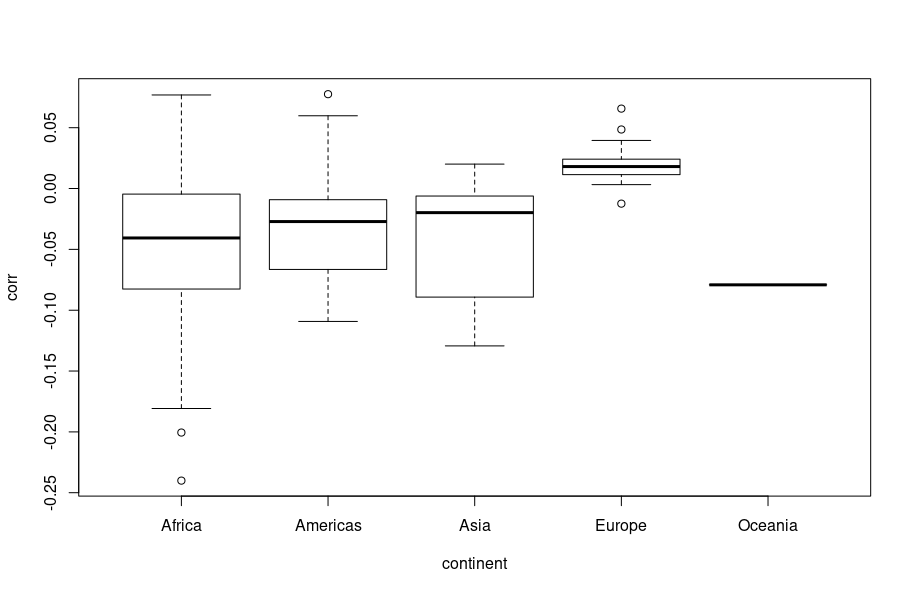
\includegraphics[scale=0.75]{images/SensitivityScoresClimate.png}
	
	Built Land \newline
	
	175 countries and 3 years matched between datasets. only 1 country gave significant result.
	
	Didn't work with built land data because there were only 3 years that matched in the dataset and only 1 country came back as having a significant relationship. \newline
	
	Pollution \newline
	
	There were only 43 countries and 16 years that matched between the datasets, and only 7 of these had significant results \newline
	
	Invasive \newline
	
	147 countries matched between datasets but the whole things a shitshow so lets ignore this one
	
	
	
	
	 
	\subsection*{Method 2: dummy variables}
	\addcontentsline{toc}{subsection}{Method 2: dummy variables}
	 
	 Africa is reference level for all models. \newline

Invasive species \newline

Intercept for Africa was statistically significantly different from zero (0.78), and no other continents had a significantly different intercept apart from Europe's which was 0.68. 

There was no significant relationship found between number of invasive species and biodiversity in Africa. Slope was not statistically significant from zero. Slopes from all other continents were not significantly different from Africa's. \newline

Pollution \newline

Intercept was statistically significant for Africa, but slope was not. Europe, Oceania and South America all had statistically significantly different intercepts from Africa but the other continents did not.

Europe and oceania's slopes were significantly different from Africa's but the other continents were not. \newline

Built Land \newline

Africa's intercept was significant but slope was not. Europe, north america and oceania all had significantly different intercepts to Africa's.

No slopes were significantly different from Africa's and therefore none were different from zero. \newline

Climate \newline

All intercepts and slopes were significantly different from each other. But I still need to correct for average temperature.
 
	 
	 
	 

    \clearpage
    
     \section*{Discussion}
     \addcontentsline{toc}{section}{Discussion}
     
     \clearpage
     
     \section*{Conclusion }
     \addcontentsline{toc}{section}{Conclusion}
     optional section
     \clearpage
    
    \section*{Data and Code Availability}
    \addcontentsline{toc}{section}{Data and Code Availability}
    Data  and  CodeAvailabilitystatement:  At  the  end  of  your  Main  text,  before  the  References section, you must provide a statement titled “Data and Code Availability”, where you name a data (e.g., Dropbox, FigShare, Zenodo, etc) and a code (e.g., Dropbox, GitHub, etc.) archive 
    20from where the data and code can be obtained that will allow replication of your results. The code may be in the form of a single script file.
    
    \clearpage
    \section*{Acknowledgements}
    \addcontentsline{toc}{section}{Acknowledgements}
    \bibliographystyle{apalike}

    \bibliography{writeup}
\end{document}